\documentclass[1p]{elsarticle_modified}
%\bibliographystyle{elsarticle-num}

%\usepackage[colorlinks]{hyperref}
%\usepackage{abbrmath_seonhwa} %\Abb, \Ascr, \Acal ,\Abf, \Afrak
\usepackage{amsfonts}
\usepackage{amssymb}
\usepackage{amsmath}
\usepackage{amsthm}
\usepackage{scalefnt}
\usepackage{amsbsy}
\usepackage{kotex}
\usepackage{caption}
\usepackage{subfig}
\usepackage{color}
\usepackage{graphicx}
\usepackage{xcolor} %% white, black, red, green, blue, cyan, magenta, yellow
\usepackage{float}
\usepackage{setspace}
\usepackage{hyperref}

\usepackage{tikz}
\usetikzlibrary{arrows}

\usepackage{multirow}
\usepackage{array} % fixed length table
\usepackage{hhline}

%%%%%%%%%%%%%%%%%%%%%
\makeatletter
\renewcommand*\env@matrix[1][\arraystretch]{%
	\edef\arraystretch{#1}%
	\hskip -\arraycolsep
	\let\@ifnextchar\new@ifnextchar
	\array{*\c@MaxMatrixCols c}}
\makeatother %https://tex.stackexchange.com/questions/14071/how-can-i-increase-the-line-spacing-in-a-matrix
%%%%%%%%%%%%%%%

\usepackage[normalem]{ulem}

\newcommand{\msout}[1]{\ifmmode\text{\sout{\ensuremath{#1}}}\else\sout{#1}\fi}
%SOURCE: \msout is \stkout macro in https://tex.stackexchange.com/questions/20609/strikeout-in-math-mode

\newcommand{\cancel}[1]{
	\ifmmode
	{\color{red}\msout{#1}}
	\else
	{\color{red}\sout{#1}}
	\fi
}

\newcommand{\add}[1]{
	{\color{blue}\uwave{#1}}
}

\newcommand{\replace}[2]{
	\ifmmode
	{\color{red}\msout{#1}}{\color{blue}\uwave{#2}}
	\else
	{\color{red}\sout{#1}}{\color{blue}\uwave{#2}}
	\fi
}

\newcommand{\Sol}{\mathcal{S}} %segment
\newcommand{\D}{D} %diagram
\newcommand{\A}{\mathcal{A}} %arc


%%%%%%%%%%%%%%%%%%%%%%%%%%%%%5 test

\def\sl{\operatorname{\textup{SL}}(2,\Cbb)}
\def\psl{\operatorname{\textup{PSL}}(2,\Cbb)}
\def\quan{\mkern 1mu \triangleright \mkern 1mu}

\theoremstyle{definition}
\newtheorem{thm}{Theorem}[section]
\newtheorem{prop}[thm]{Proposition}
\newtheorem{lem}[thm]{Lemma}
\newtheorem{ques}[thm]{Question}
\newtheorem{cor}[thm]{Corollary}
\newtheorem{defn}[thm]{Definition}
\newtheorem{exam}[thm]{Example}
\newtheorem{rmk}[thm]{Remark}
\newtheorem{alg}[thm]{Algorithm}

\newcommand{\I}{\sqrt{-1}}
\begin{document}

%\begin{frontmatter}
%
%\title{Boundary parabolic representations of knots up to 8 crossings}
%
%%% Group authors per affiliation:
%\author{Yunhi Cho} 
%\address{Department of Mathematics, University of Seoul, Seoul, Korea}
%\ead{yhcho@uos.ac.kr}
%
%
%\author{Seonhwa Kim} %\fnref{s_kim}}
%\address{Center for Geometry and Physics, Institute for Basic Science, Pohang, 37673, Korea}
%\ead{ryeona17@ibs.re.kr}
%
%\author{Hyuk Kim}
%\address{Department of Mathematical Sciences, Seoul National University, Seoul 08826, Korea}
%\ead{hyukkim@snu.ac.kr}
%
%\author{Seokbeom Yoon}
%\address{Department of Mathematical Sciences, Seoul National University, Seoul, 08826,  Korea}
%\ead{sbyoon15@snu.ac.kr}
%
%\begin{abstract}
%We find all boundary parabolic representation of knots up to 8 crossings.
%
%\end{abstract}
%\begin{keyword}
%    \MSC[2010] 57M25 
%\end{keyword}
%
%\end{frontmatter}

%\linenumbers
%\tableofcontents
%
\newcommand\colored[1]{\textcolor{white}{\rule[-0.35ex]{0.8em}{1.4ex}}\kern-0.8em\color{red} #1}%
%\newcommand\colored[1]{\textcolor{white}{ #1}\kern-2.17ex	\textcolor{white}{ #1}\kern-1.81ex	\textcolor{white}{ #1}\kern-2.15ex\color{red}#1	}

{\Large $\underline{12n_{0017}~(K12n_{0017})}$}

\setlength{\tabcolsep}{10pt}
\renewcommand{\arraystretch}{1.6}
\vspace{1cm}\begin{tabular}{m{100pt}>{\centering\arraybackslash}m{274pt}}
\multirow{5}{120pt}{
	\centering
	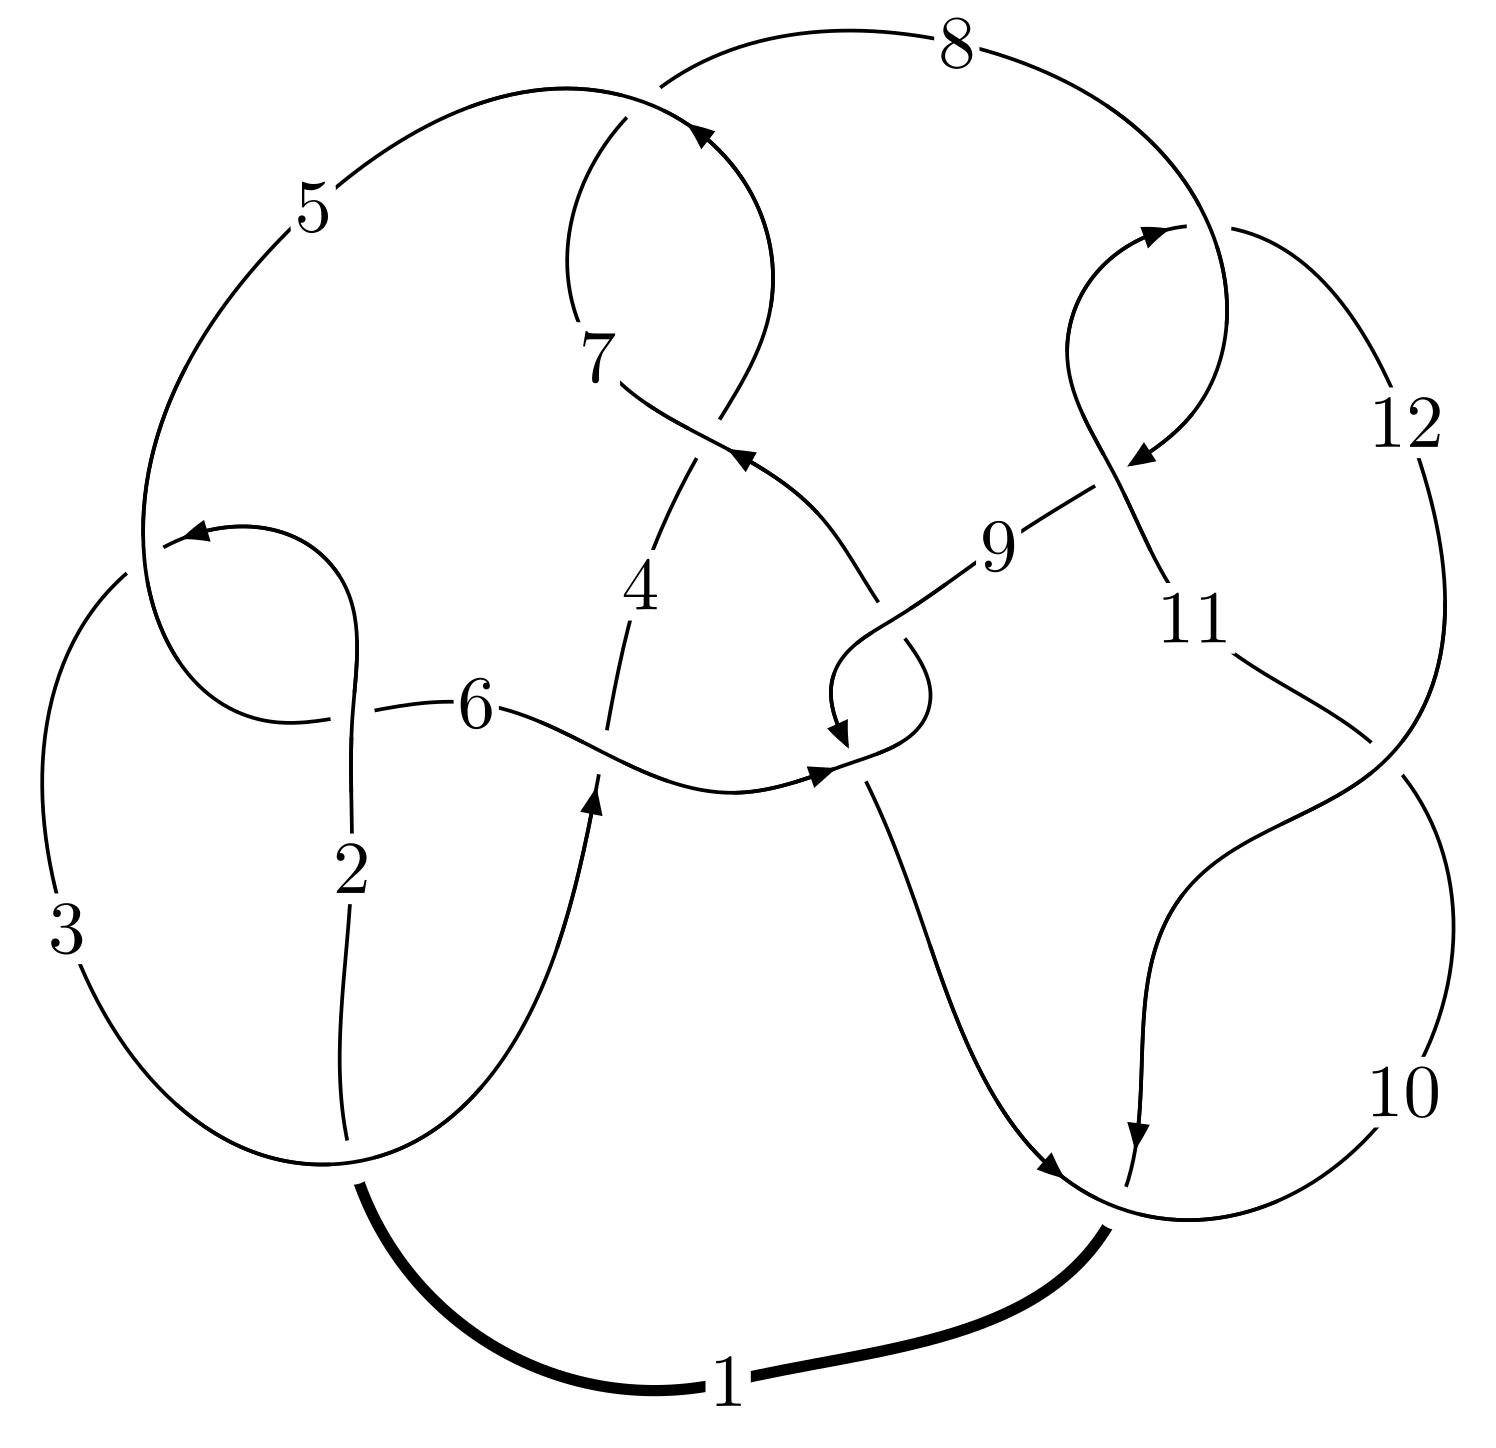
\includegraphics[width=112pt]{../../../GIT/diagram.site/Diagrams/png/2106_12n_0017.png}\\
\ \ \ A knot diagram\footnotemark}&
\allowdisplaybreaks
\textbf{Linearized knot diagam} \\
\cline{2-2}
 &
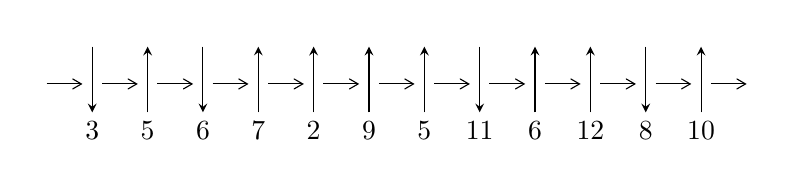
\begin{tikzpicture}[x=20pt, y=17pt]
	% nodes
	\node (C0) at (0, 0) {};
	\node (C1) at (1, 0) {};
	\node (C1U) at (1, +1) {};
	\node (C1D) at (1, -1) {3};

	\node (C2) at (2, 0) {};
	\node (C2U) at (2, +1) {};
	\node (C2D) at (2, -1) {5};

	\node (C3) at (3, 0) {};
	\node (C3U) at (3, +1) {};
	\node (C3D) at (3, -1) {6};

	\node (C4) at (4, 0) {};
	\node (C4U) at (4, +1) {};
	\node (C4D) at (4, -1) {7};

	\node (C5) at (5, 0) {};
	\node (C5U) at (5, +1) {};
	\node (C5D) at (5, -1) {2};

	\node (C6) at (6, 0) {};
	\node (C6U) at (6, +1) {};
	\node (C6D) at (6, -1) {9};

	\node (C7) at (7, 0) {};
	\node (C7U) at (7, +1) {};
	\node (C7D) at (7, -1) {5};

	\node (C8) at (8, 0) {};
	\node (C8U) at (8, +1) {};
	\node (C8D) at (8, -1) {11};

	\node (C9) at (9, 0) {};
	\node (C9U) at (9, +1) {};
	\node (C9D) at (9, -1) {6};

	\node (C10) at (10, 0) {};
	\node (C10U) at (10, +1) {};
	\node (C10D) at (10, -1) {12};

	\node (C11) at (11, 0) {};
	\node (C11U) at (11, +1) {};
	\node (C11D) at (11, -1) {8};

	\node (C12) at (12, 0) {};
	\node (C12U) at (12, +1) {};
	\node (C12D) at (12, -1) {10};
	\node (C13) at (13, 0) {};

	% arrows
	\draw[->,>={angle 60}]
	(C0) edge (C1) (C1) edge (C2) (C2) edge (C3) (C3) edge (C4) (C4) edge (C5) (C5) edge (C6) (C6) edge (C7) (C7) edge (C8) (C8) edge (C9) (C9) edge (C10) (C10) edge (C11) (C11) edge (C12) (C12) edge (C13) ;	\draw[->,>=stealth]
	(C1U) edge (C1D) (C2D) edge (C2U) (C3U) edge (C3D) (C4D) edge (C4U) (C5D) edge (C5U) (C6D) edge (C6U) (C7D) edge (C7U) (C8U) edge (C8D) (C9D) edge (C9U) (C10D) edge (C10U) (C11U) edge (C11D) (C12D) edge (C12U) ;
	\end{tikzpicture} \\
\hhline{~~} \\& 
\textbf{Solving Sequence} \\ \cline{2-2} 
 &
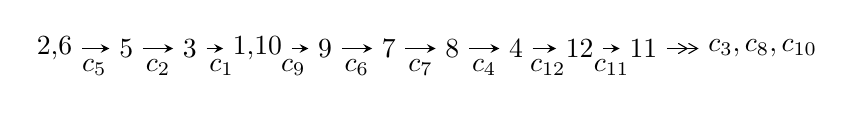
\begin{tikzpicture}[x=23pt, y=7pt]
	% node
	\node (A0) at (-1/8, 0) {2,6};
	\node (A1) at (1, 0) {5};
	\node (A2) at (2, 0) {3};
	\node (A3) at (49/16, 0) {1,10};
	\node (A4) at (33/8, 0) {9};
	\node (A5) at (41/8, 0) {7};
	\node (A6) at (49/8, 0) {8};
	\node (A7) at (57/8, 0) {4};
	\node (A8) at (65/8, 0) {12};
	\node (A9) at (73/8, 0) {11};
	\node (C1) at (1/2, -1) {$c_{5}$};
	\node (C2) at (3/2, -1) {$c_{2}$};
	\node (C3) at (5/2, -1) {$c_{1}$};
	\node (C4) at (29/8, -1) {$c_{9}$};
	\node (C5) at (37/8, -1) {$c_{6}$};
	\node (C6) at (45/8, -1) {$c_{7}$};
	\node (C7) at (53/8, -1) {$c_{4}$};
	\node (C8) at (61/8, -1) {$c_{12}$};
	\node (C9) at (69/8, -1) {$c_{11}$};
	\node (A10) at (11, 0) {$c_{3},c_{8},c_{10}$};

	% edge
	\draw[->,>=stealth]	
	(A0) edge (A1) (A1) edge (A2) (A2) edge (A3) (A3) edge (A4) (A4) edge (A5) (A5) edge (A6) (A6) edge (A7) (A7) edge (A8) (A8) edge (A9) ;
	\draw[->>,>={angle 60}]	
	(A9) edge (A10);
\end{tikzpicture} \\ 

\end{tabular} \\

\footnotetext{
The image of knot diagram is generated by the software ``\textbf{Draw programme}" developed by Andrew Bartholomew(\url{http://www.layer8.co.uk/maths/draw/index.htm\#Running-draw}), where we modified some parts for our purpose(\url{https://github.com/CATsTAILs/LinksPainter}).
}\phantom \\ \newline 
\centering \textbf{Ideals for irreducible components\footnotemark of $X_{\text{par}}$} 
 
\begin{align*}
I^u_{1}&=\langle 
-4.18594\times10^{34} u^{52}-2.07414\times10^{35} u^{51}+\cdots+1.22009\times10^{34} b+4.27515\times10^{34},\\
\phantom{I^u_{1}}&\phantom{= \langle  }-5.11228\times10^{32} u^{52}-1.97357\times10^{33} u^{51}+\cdots+1.82103\times10^{32} a-9.15657\times10^{32},\;u^{53}+5 u^{52}+\cdots-9 u-1\rangle \\
I^u_{2}&=\langle 
- a^3 u- a^3-3 a^2- a u+3 b+2 a+u+4,\;a^4- a^3 u+3 a^3- a^2 u+a^2-4 a- u-3,\;u^2- u+1\rangle \\
\\
\end{align*}
\raggedright * 2 irreducible components of $\dim_{\mathbb{C}}=0$, with total 61 representations.\\
\footnotetext{All coefficients of polynomials are rational numbers. But the coefficients are sometimes approximated in decimal forms when there is not enough margin.}
\newpage
\renewcommand{\arraystretch}{1}
\centering \section*{I. $I^u_{1}= \langle -4.19\times10^{34} u^{52}-2.07\times10^{35} u^{51}+\cdots+1.22\times10^{34} b+4.28\times10^{34},\;-5.11\times10^{32} u^{52}-1.97\times10^{33} u^{51}+\cdots+1.82\times10^{32} a-9.16\times10^{32},\;u^{53}+5 u^{52}+\cdots-9 u-1 \rangle$}
\flushleft \textbf{(i) Arc colorings}\\
\begin{tabular}{m{7pt} m{180pt} m{7pt} m{180pt} }
\flushright $a_{2}=$&$\begin{pmatrix}0\\u\end{pmatrix}$ \\
\flushright $a_{6}=$&$\begin{pmatrix}1\\0\end{pmatrix}$ \\
\flushright $a_{5}=$&$\begin{pmatrix}1\\u^2\end{pmatrix}$ \\
\flushright $a_{3}=$&$\begin{pmatrix}u\\u^3+u\end{pmatrix}$ \\
\flushright $a_{1}=$&$\begin{pmatrix}u^3\\u^5+u^3+u\end{pmatrix}$ \\
\flushright $a_{10}=$&$\begin{pmatrix}2.80735 u^{52}+10.8376 u^{51}+\cdots-0.444267 u+5.02822\\3.43084 u^{52}+16.9999 u^{51}+\cdots-34.1145 u-3.50395\end{pmatrix}$ \\
\flushright $a_{9}=$&$\begin{pmatrix}-0.623488 u^{52}-6.16226 u^{51}+\cdots+33.6702 u+8.53217\\3.43084 u^{52}+16.9999 u^{51}+\cdots-34.1145 u-3.50395\end{pmatrix}$ \\
\flushright $a_{7}=$&$\begin{pmatrix}-1.75032 u^{52}-0.890320 u^{51}+\cdots-10.7679 u-3.13567\\-6.83122 u^{52}-35.1862 u^{51}+\cdots+71.7880 u+8.58154\end{pmatrix}$ \\
\flushright $a_{8}=$&$\begin{pmatrix}1.59554 u^{52}+9.62066 u^{51}+\cdots-7.98101 u-2.41540\\-1.76578 u^{52}-8.80291 u^{51}+\cdots+19.1693 u+2.36325\end{pmatrix}$ \\
\flushright $a_{4}=$&$\begin{pmatrix}- u^3\\u^3+u\end{pmatrix}$ \\
\flushright $a_{12}=$&$\begin{pmatrix}4.55627 u^{52}+20.9187 u^{51}+\cdots-49.1860 u-2.25218\\1.76578 u^{52}+8.80291 u^{51}+\cdots-19.1693 u-2.36325\end{pmatrix}$ \\
\flushright $a_{11}=$&$\begin{pmatrix}1.71105 u^{52}+5.75864 u^{51}+\cdots-19.5378 u+3.68527\\2.74059 u^{52}+13.6878 u^{51}+\cdots-30.0115 u-3.36198\end{pmatrix}$\\&\end{tabular}
\flushleft \textbf{(ii) Obstruction class $= -1$}\\~\\
\flushleft \textbf{(iii) Cusp Shapes $= -5.35104 u^{52}-25.5532 u^{51}+\cdots+78.3747 u+11.0743$}\\~\\
\newpage\renewcommand{\arraystretch}{1}
\flushleft \textbf{(iv) u-Polynomials at the component}\newline \\
\begin{tabular}{m{50pt}|m{274pt}}
Crossings & \hspace{64pt}u-Polynomials at each crossing \\
\hline $$\begin{aligned}c_{1}\end{aligned}$$&$\begin{aligned}
&u^{53}+15 u^{52}+\cdots-9 u-1
\end{aligned}$\\
\hline $$\begin{aligned}c_{2},c_{5}\end{aligned}$$&$\begin{aligned}
&u^{53}+5 u^{52}+\cdots-9 u-1
\end{aligned}$\\
\hline $$\begin{aligned}c_{3}\end{aligned}$$&$\begin{aligned}
&u^{53}-5 u^{52}+\cdots-2302791 u-148289
\end{aligned}$\\
\hline $$\begin{aligned}c_{4},c_{7}\end{aligned}$$&$\begin{aligned}
&u^{53}+5 u^{52}+\cdots-1664 u-256
\end{aligned}$\\
\hline $$\begin{aligned}c_{6},c_{9}\end{aligned}$$&$\begin{aligned}
&u^{53}+3 u^{52}+\cdots-3 u-1
\end{aligned}$\\
\hline $$\begin{aligned}c_{8},c_{11}\end{aligned}$$&$\begin{aligned}
&u^{53}-3 u^{52}+\cdots+5 u-1
\end{aligned}$\\
\hline $$\begin{aligned}c_{10},c_{12}\end{aligned}$$&$\begin{aligned}
&u^{53}-21 u^{52}+\cdots- u+1
\end{aligned}$\\
\hline
\end{tabular}\\~\\
\newpage\renewcommand{\arraystretch}{1}
\flushleft \textbf{(v) Riley Polynomials at the component}\newline \\
\begin{tabular}{m{50pt}|m{274pt}}
Crossings & \hspace{64pt}Riley Polynomials at each crossing \\
\hline $$\begin{aligned}c_{1}\end{aligned}$$&$\begin{aligned}
&y^{53}+51 y^{52}+\cdots-4269 y-1
\end{aligned}$\\
\hline $$\begin{aligned}c_{2},c_{5}\end{aligned}$$&$\begin{aligned}
&y^{53}+15 y^{52}+\cdots-9 y-1
\end{aligned}$\\
\hline $$\begin{aligned}c_{3}\end{aligned}$$&$\begin{aligned}
&y^{53}+87 y^{52}+\cdots-708900293913 y-21989627521
\end{aligned}$\\
\hline $$\begin{aligned}c_{4},c_{7}\end{aligned}$$&$\begin{aligned}
&y^{53}-45 y^{52}+\cdots-606208 y-65536
\end{aligned}$\\
\hline $$\begin{aligned}c_{6},c_{9}\end{aligned}$$&$\begin{aligned}
&y^{53}+5 y^{52}+\cdots- y-1
\end{aligned}$\\
\hline $$\begin{aligned}c_{8},c_{11}\end{aligned}$$&$\begin{aligned}
&y^{53}+21 y^{52}+\cdots- y-1
\end{aligned}$\\
\hline $$\begin{aligned}c_{10},c_{12}\end{aligned}$$&$\begin{aligned}
&y^{53}+25 y^{52}+\cdots-77 y-1
\end{aligned}$\\
\hline
\end{tabular}\\~\\
\newpage\flushleft \textbf{(vi) Complex Volumes and Cusp Shapes}
$$\begin{array}{c|c|c}  
\text{Solutions to }I^u_{1}& \I (\text{vol} + \sqrt{-1}CS) & \text{Cusp shape}\\
 \hline 
\begin{aligned}
u &= \phantom{-}0.530308 + 0.891641 I \\
a &= -1.41610 - 2.34002 I \\
b &= -0.227413 + 0.365967 I\end{aligned}
 & \phantom{-}0.156968 + 0.305979 I & -9.1267 + 31.8061 I \\ \hline\begin{aligned}
u &= \phantom{-}0.530308 - 0.891641 I \\
a &= -1.41610 + 2.34002 I \\
b &= -0.227413 - 0.365967 I\end{aligned}
 & \phantom{-}0.156968 - 0.305979 I & -9.1267 - 31.8061 I \\ \hline\begin{aligned}
u &= \phantom{-}0.550027 + 0.789290 I \\
a &= \phantom{-}0.66997 + 2.28557 I \\
b &= \phantom{-}0.074147 - 0.510318 I\end{aligned}
 & \phantom{-}0.47806 + 4.00723 I & -10.14274 - 8.52943 I \\ \hline\begin{aligned}
u &= \phantom{-}0.550027 - 0.789290 I \\
a &= \phantom{-}0.66997 - 2.28557 I \\
b &= \phantom{-}0.074147 + 0.510318 I\end{aligned}
 & \phantom{-}0.47806 - 4.00723 I & -10.14274 + 8.52943 I \\ \hline\begin{aligned}
u &= \phantom{-}0.290660 + 0.872671 I \\
a &= -1.38678 - 1.24113 I \\
b &= -0.646642 + 0.233451 I\end{aligned}
 & -0.90313 + 4.01726 I & \phantom{-}5.20804 - 5.06978 I \\ \hline\begin{aligned}
u &= \phantom{-}0.290660 - 0.872671 I \\
a &= -1.38678 + 1.24113 I \\
b &= -0.646642 - 0.233451 I\end{aligned}
 & -0.90313 - 4.01726 I & \phantom{-}5.20804 + 5.06978 I \\ \hline\begin{aligned}
u &= \phantom{-}1.056180 + 0.236014 I \\
a &= -0.594933 - 0.033166 I \\
b &= -0.768107 - 0.046948 I\end{aligned}
 & \phantom{-}3.64081 + 3.04661 I & \phantom{-}13.4424 - 4.7932 I \\ \hline\begin{aligned}
u &= \phantom{-}1.056180 - 0.236014 I \\
a &= -0.594933 + 0.033166 I \\
b &= -0.768107 + 0.046948 I\end{aligned}
 & \phantom{-}3.64081 - 3.04661 I & \phantom{-}13.4424 + 4.7932 I \\ \hline\begin{aligned}
u &= \phantom{-}0.657790 + 0.921515 I \\
a &= -1.023740 + 0.420502 I \\
b &= -0.553170 - 0.255009 I\end{aligned}
 & \phantom{-}0.62571 + 2.57123 I & \phantom{-0.000000 } 0 \\ \hline\begin{aligned}
u &= \phantom{-}0.657790 - 0.921515 I \\
a &= -1.023740 - 0.420502 I \\
b &= -0.553170 + 0.255009 I\end{aligned}
 & \phantom{-}0.62571 - 2.57123 I & \phantom{-0.000000 } 0\\
 \hline 
 \end{array}$$\newpage$$\begin{array}{c|c|c}  
\text{Solutions to }I^u_{1}& \I (\text{vol} + \sqrt{-1}CS) & \text{Cusp shape}\\
 \hline 
\begin{aligned}
u &= \phantom{-}0.169703 + 0.847189 I \\
a &= -0.573410 - 1.128960 I \\
b &= \phantom{-}0.220478 + 0.766514 I\end{aligned}
 & -1.59631 + 1.76854 I & -2.74640 - 4.48451 I \\ \hline\begin{aligned}
u &= \phantom{-}0.169703 - 0.847189 I \\
a &= -0.573410 + 1.128960 I \\
b &= \phantom{-}0.220478 - 0.766514 I\end{aligned}
 & -1.59631 - 1.76854 I & -2.74640 + 4.48451 I \\ \hline\begin{aligned}
u &= -0.359167 + 0.783757 I \\
a &= -1.60327 + 0.04327 I \\
b &= -0.01818 + 1.50451 I\end{aligned}
 & -7.06670 + 1.57178 I & -4.33706 - 7.74502 I \\ \hline\begin{aligned}
u &= -0.359167 - 0.783757 I \\
a &= -1.60327 - 0.04327 I \\
b &= -0.01818 - 1.50451 I\end{aligned}
 & -7.06670 - 1.57178 I & -4.33706 + 7.74502 I \\ \hline\begin{aligned}
u &= -0.409008 + 0.741183 I \\
a &= \phantom{-}1.80767 - 0.00417 I \\
b &= \phantom{-}0.22475 - 1.53329 I\end{aligned}
 & -6.87601 - 4.70786 I & -1.13106 - 3.85165 I \\ \hline\begin{aligned}
u &= -0.409008 - 0.741183 I \\
a &= \phantom{-}1.80767 + 0.00417 I \\
b &= \phantom{-}0.22475 + 1.53329 I\end{aligned}
 & -6.87601 + 4.70786 I & -1.13106 + 3.85165 I \\ \hline\begin{aligned}
u &= -0.923392 + 0.708125 I \\
a &= \phantom{-}0.826229 + 0.812255 I \\
b &= \phantom{-}1.15258 + 0.92886 I\end{aligned}
 & \phantom{-}4.90426 + 3.27952 I & \phantom{-0.000000 } 0 \\ \hline\begin{aligned}
u &= -0.923392 - 0.708125 I \\
a &= \phantom{-}0.826229 - 0.812255 I \\
b &= \phantom{-}1.15258 - 0.92886 I\end{aligned}
 & \phantom{-}4.90426 - 3.27952 I & \phantom{-0.000000 } 0 \\ \hline\begin{aligned}
u &= -0.809353 + 0.881663 I \\
a &= \phantom{-}0.531942 + 0.908624 I \\
b &= \phantom{-}1.20306 + 1.02356 I\end{aligned}
 & \phantom{-}4.15839 - 1.32183 I & \phantom{-0.000000 } 0 \\ \hline\begin{aligned}
u &= -0.809353 - 0.881663 I \\
a &= \phantom{-}0.531942 - 0.908624 I \\
b &= \phantom{-}1.20306 - 1.02356 I\end{aligned}
 & \phantom{-}4.15839 + 1.32183 I & \phantom{-0.000000 } 0\\
 \hline 
 \end{array}$$\newpage$$\begin{array}{c|c|c}  
\text{Solutions to }I^u_{1}& \I (\text{vol} + \sqrt{-1}CS) & \text{Cusp shape}\\
 \hline 
\begin{aligned}
u &= \phantom{-}0.963077 + 0.716560 I \\
a &= \phantom{-}0.748110 - 0.046980 I \\
b &= \phantom{-}0.724122 + 0.163979 I\end{aligned}
 & \phantom{-}3.13131 + 0.47040 I & \phantom{-0.000000 } 0 \\ \hline\begin{aligned}
u &= \phantom{-}0.963077 - 0.716560 I \\
a &= \phantom{-}0.748110 + 0.046980 I \\
b &= \phantom{-}0.724122 - 0.163979 I\end{aligned}
 & \phantom{-}3.13131 - 0.47040 I & \phantom{-0.000000 } 0 \\ \hline\begin{aligned}
u &= -0.848949 + 0.856511 I \\
a &= -1.69721 - 0.38788 I \\
b &= -0.99863 + 1.18800 I\end{aligned}
 & \phantom{-}6.21091 + 1.13505 I & \phantom{-0.000000 } 0 \\ \hline\begin{aligned}
u &= -0.848949 - 0.856511 I \\
a &= -1.69721 + 0.38788 I \\
b &= -0.99863 - 1.18800 I\end{aligned}
 & \phantom{-}6.21091 - 1.13505 I & \phantom{-0.000000 } 0 \\ \hline\begin{aligned}
u &= -0.997021 + 0.686901 I \\
a &= -0.854814 - 0.725692 I \\
b &= -1.12564 - 0.93321 I\end{aligned}
 & \phantom{-}7.01799 + 8.93611 I & \phantom{-0.000000 } 0 \\ \hline\begin{aligned}
u &= -0.997021 - 0.686901 I \\
a &= -0.854814 + 0.725692 I \\
b &= -1.12564 + 0.93321 I\end{aligned}
 & \phantom{-}7.01799 - 8.93611 I & \phantom{-0.000000 } 0 \\ \hline\begin{aligned}
u &= -0.800905 + 0.909129 I \\
a &= \phantom{-}1.72367 + 0.46790 I \\
b &= \phantom{-}1.04239 - 1.19652 I\end{aligned}
 & \phantom{-}4.07249 - 4.71363 I & \phantom{-0.000000 } 0 \\ \hline\begin{aligned}
u &= -0.800905 - 0.909129 I \\
a &= \phantom{-}1.72367 - 0.46790 I \\
b &= \phantom{-}1.04239 + 1.19652 I\end{aligned}
 & \phantom{-}4.07249 + 4.71363 I & \phantom{-0.000000 } 0 \\ \hline\begin{aligned}
u &= \phantom{-}0.190036 + 1.206100 I \\
a &= -0.014657 - 0.532586 I \\
b &= \phantom{-}0.543932 + 0.735641 I\end{aligned}
 & -2.94216 + 2.73108 I & \phantom{-0.000000 } 0 \\ \hline\begin{aligned}
u &= \phantom{-}0.190036 - 1.206100 I \\
a &= -0.014657 + 0.532586 I \\
b &= \phantom{-}0.543932 - 0.735641 I\end{aligned}
 & -2.94216 - 2.73108 I & \phantom{-0.000000 } 0\\
 \hline 
 \end{array}$$\newpage$$\begin{array}{c|c|c}  
\text{Solutions to }I^u_{1}& \I (\text{vol} + \sqrt{-1}CS) & \text{Cusp shape}\\
 \hline 
\begin{aligned}
u &= \phantom{-}0.167242 + 0.748310 I \\
a &= \phantom{-}1.20707 + 1.23679 I \\
b &= \phantom{-}0.772219 - 0.132719 I\end{aligned}
 & -1.23355 - 0.85670 I & \phantom{-}1.99397 + 0.77147 I \\ \hline\begin{aligned}
u &= \phantom{-}0.167242 - 0.748310 I \\
a &= \phantom{-}1.20707 - 1.23679 I \\
b &= \phantom{-}0.772219 + 0.132719 I\end{aligned}
 & -1.23355 + 0.85670 I & \phantom{-}1.99397 - 0.77147 I \\ \hline\begin{aligned}
u &= \phantom{-}0.593122 + 1.098860 I \\
a &= -0.640887 + 0.592926 I \\
b &= -0.568895 - 0.414061 I\end{aligned}
 & \phantom{-}0.79815 + 2.64733 I & \phantom{-0.000000 } 0 \\ \hline\begin{aligned}
u &= \phantom{-}0.593122 - 1.098860 I \\
a &= -0.640887 - 0.592926 I \\
b &= -0.568895 + 0.414061 I\end{aligned}
 & \phantom{-}0.79815 - 2.64733 I & \phantom{-0.000000 } 0 \\ \hline\begin{aligned}
u &= -0.816554 + 0.945782 I \\
a &= -0.448825 - 0.835890 I \\
b &= -1.17212 - 1.05145 I\end{aligned}
 & \phantom{-}5.93083 - 7.33894 I & \phantom{-0.000000 } 0 \\ \hline\begin{aligned}
u &= -0.816554 - 0.945782 I \\
a &= -0.448825 + 0.835890 I \\
b &= -1.17212 + 1.05145 I\end{aligned}
 & \phantom{-}5.93083 + 7.33894 I & \phantom{-0.000000 } 0 \\ \hline\begin{aligned}
u &= -0.938500 + 0.838979 I \\
a &= -0.667637 - 0.761297 I \\
b &= -1.15180 - 0.97924 I\end{aligned}
 & \phantom{-}11.01260 + 0.70068 I & \phantom{-0.000000 } 0 \\ \hline\begin{aligned}
u &= -0.938500 - 0.838979 I \\
a &= -0.667637 + 0.761297 I \\
b &= -1.15180 + 0.97924 I\end{aligned}
 & \phantom{-}11.01260 - 0.70068 I & \phantom{-0.000000 } 0 \\ \hline\begin{aligned}
u &= -0.781108 + 1.058600 I \\
a &= \phantom{-}1.62355 + 0.62236 I \\
b &= \phantom{-}1.09267 - 1.11554 I\end{aligned}
 & \phantom{-}3.80915 - 9.57151 I & \phantom{-0.000000 } 0 \\ \hline\begin{aligned}
u &= -0.781108 - 1.058600 I \\
a &= \phantom{-}1.62355 - 0.62236 I \\
b &= \phantom{-}1.09267 + 1.11554 I\end{aligned}
 & \phantom{-}3.80915 + 9.57151 I & \phantom{-0.000000 } 0\\
 \hline 
 \end{array}$$\newpage$$\begin{array}{c|c|c}  
\text{Solutions to }I^u_{1}& \I (\text{vol} + \sqrt{-1}CS) & \text{Cusp shape}\\
 \hline 
\begin{aligned}
u &= -0.855619 + 1.002320 I \\
a &= -1.61140 - 0.52084 I \\
b &= -1.04937 + 1.13619 I\end{aligned}
 & \phantom{-}10.48550 - 7.29514 I & \phantom{-0.000000 } 0 \\ \hline\begin{aligned}
u &= -0.855619 - 1.002320 I \\
a &= -1.61140 + 0.52084 I \\
b &= -1.04937 - 1.13619 I\end{aligned}
 & \phantom{-}10.48550 + 7.29514 I & \phantom{-0.000000 } 0 \\ \hline\begin{aligned}
u &= \phantom{-}0.276293 + 1.310550 I \\
a &= -0.145590 + 0.459150 I \\
b &= -0.617657 - 0.677073 I\end{aligned}
 & -1.79792 + 7.60628 I & \phantom{-0.000000 } 0 \\ \hline\begin{aligned}
u &= \phantom{-}0.276293 - 1.310550 I \\
a &= -0.145590 - 0.459150 I \\
b &= -0.617657 + 0.677073 I\end{aligned}
 & -1.79792 - 7.60628 I & \phantom{-0.000000 } 0 \\ \hline\begin{aligned}
u &= \phantom{-}0.651246\phantom{ +0.000000I} \\
a &= \phantom{-}0.347416\phantom{ +0.000000I} \\
b &= \phantom{-}0.701762\phantom{ +0.000000I}\end{aligned}
 & \phantom{-}1.38715\phantom{ +0.000000I} & \phantom{-}7.24480\phantom{ +0.000000I} \\ \hline\begin{aligned}
u &= -0.797265 + 1.097860 I \\
a &= -1.57835 - 0.63310 I \\
b &= -1.08229 + 1.09516 I\end{aligned}
 & \phantom{-}5.7123 - 15.4835 I & \phantom{-0.000000 } 0 \\ \hline\begin{aligned}
u &= -0.797265 - 1.097860 I \\
a &= -1.57835 + 0.63310 I \\
b &= -1.08229 - 1.09516 I\end{aligned}
 & \phantom{-}5.7123 + 15.4835 I & \phantom{-0.000000 } 0 \\ \hline\begin{aligned}
u &= \phantom{-}0.884439 + 1.048670 I \\
a &= \phantom{-}0.701048 - 0.259116 I \\
b &= \phantom{-}0.705424 + 0.300411 I\end{aligned}
 & \phantom{-}2.15584 + 6.28914 I & \phantom{-0.000000 } 0 \\ \hline\begin{aligned}
u &= \phantom{-}0.884439 - 1.048670 I \\
a &= \phantom{-}0.701048 + 0.259116 I \\
b &= \phantom{-}0.705424 - 0.300411 I\end{aligned}
 & \phantom{-}2.15584 - 6.28914 I & \phantom{-0.000000 } 0 \\ \hline\begin{aligned}
u &= \phantom{-}0.289494 + 0.414333 I \\
a &= \phantom{-}1.16272 + 2.27371 I \\
b &= \phantom{-}0.033058 - 0.698327 I\end{aligned}
 & \phantom{-}0.54607 - 1.46734 I & \phantom{-}1.60005 + 1.62915 I\\
 \hline 
 \end{array}$$\newpage$$\begin{array}{c|c|c}  
\text{Solutions to }I^u_{1}& \I (\text{vol} + \sqrt{-1}CS) & \text{Cusp shape}\\
 \hline 
\begin{aligned}
u &= \phantom{-}0.289494 - 0.414333 I \\
a &= \phantom{-}1.16272 - 2.27371 I \\
b &= \phantom{-}0.033058 + 0.698327 I\end{aligned}
 & \phantom{-}0.54607 + 1.46734 I & \phantom{-}1.60005 - 1.62915 I \\ \hline\begin{aligned}
u &= -0.107152 + 0.100700 I \\
a &= \phantom{-}5.08191 + 0.12392 I \\
b &= \phantom{-}0.340195 - 0.558279 I\end{aligned}
 & \phantom{-}0.33530 - 1.50733 I & \phantom{-}2.98224 + 4.24130 I \\ \hline\begin{aligned}
u &= -0.107152 - 0.100700 I \\
a &= \phantom{-}5.08191 - 0.12392 I \\
b &= \phantom{-}0.340195 + 0.558279 I\end{aligned}
 & \phantom{-}0.33530 + 1.50733 I & \phantom{-}2.98224 - 4.24130 I\\
 \hline 
 \end{array}$$\newpage\newpage\renewcommand{\arraystretch}{1}
\centering \section*{II. $I^u_{2}= \langle - a^3 u- a^3-3 a^2- a u+3 b+2 a+u+4,\;a^4- a^3 u+3 a^3- a^2 u+a^2-4 a- u-3,\;u^2- u+1 \rangle$}
\flushleft \textbf{(i) Arc colorings}\\
\begin{tabular}{m{7pt} m{180pt} m{7pt} m{180pt} }
\flushright $a_{2}=$&$\begin{pmatrix}0\\u\end{pmatrix}$ \\
\flushright $a_{6}=$&$\begin{pmatrix}1\\0\end{pmatrix}$ \\
\flushright $a_{5}=$&$\begin{pmatrix}1\\u-1\end{pmatrix}$ \\
\flushright $a_{3}=$&$\begin{pmatrix}u\\u-1\end{pmatrix}$ \\
\flushright $a_{1}=$&$\begin{pmatrix}-1\\0\end{pmatrix}$ \\
\flushright $a_{10}=$&$\begin{pmatrix}a\\\frac{1}{3} a^3 u+\frac{1}{3} a u+\cdots-\frac{2}{3} a-\frac{4}{3}\end{pmatrix}$ \\
\flushright $a_{9}=$&$\begin{pmatrix}-\frac{1}{3} a^3 u-\frac{1}{3} a u+\cdots+\frac{5}{3} a+\frac{4}{3}\\\frac{1}{3} a^3 u+\frac{1}{3} a u+\cdots-\frac{2}{3} a-\frac{4}{3}\end{pmatrix}$ \\
\flushright $a_{7}=$&$\begin{pmatrix}-\frac{1}{3} a^3 u-\frac{4}{3} a^2 u+\cdots- a-\frac{4}{3}\\\frac{2}{3} a^3 u+\frac{2}{3} a^2 u+\cdots+a+\frac{5}{3}\end{pmatrix}$ \\
\flushright $a_{8}=$&$\begin{pmatrix}-\frac{1}{3} a^3 u-\frac{4}{3} a^2 u+\cdots- a-\frac{4}{3}\\\frac{2}{3} a^3 u+\frac{2}{3} a^2 u+\cdots+a+\frac{5}{3}\end{pmatrix}$ \\
\flushright $a_{4}=$&$\begin{pmatrix}1\\u-1\end{pmatrix}$ \\
\flushright $a_{12}=$&$\begin{pmatrix}\frac{1}{3} a^3 u-\frac{2}{3} a^2 u+\cdots+\frac{4}{3} a^2-\frac{5}{3}\\\frac{2}{3} a^3 u+\frac{2}{3} a^2 u+\cdots+a+\frac{5}{3}\end{pmatrix}$ \\
\flushright $a_{11}=$&$\begin{pmatrix}\frac{4}{3} a^3 u+\frac{4}{3} a^2 u+\cdots+\frac{1}{3} a^2+\frac{1}{3}\\-\frac{1}{3} a^3 u-\frac{1}{3} a^2 u+\cdots+a+\frac{2}{3}\end{pmatrix}$\\&\end{tabular}
\flushleft \textbf{(ii) Obstruction class $= 1$}\\~\\
\flushleft \textbf{(iii) Cusp Shapes $= -\frac{1}{3} a^3 u+\frac{5}{3} a^3-3 a^2 u+4 a^2+\frac{5}{3} a u-\frac{7}{3} a-\frac{17}{3} u+\frac{4}{3}$}\\~\\
\newpage\renewcommand{\arraystretch}{1}
\flushleft \textbf{(iv) u-Polynomials at the component}\newline \\
\begin{tabular}{m{50pt}|m{274pt}}
Crossings & \hspace{64pt}u-Polynomials at each crossing \\
\hline $$\begin{aligned}c_{1},c_{3},c_{5}\end{aligned}$$&$\begin{aligned}
&(u^2- u+1)^4
\end{aligned}$\\
\hline $$\begin{aligned}c_{2}\end{aligned}$$&$\begin{aligned}
&(u^2+u+1)^4
\end{aligned}$\\
\hline $$\begin{aligned}c_{4},c_{7}\end{aligned}$$&$\begin{aligned}
&u^8
\end{aligned}$\\
\hline $$\begin{aligned}c_{6},c_{10}\end{aligned}$$&$\begin{aligned}
&(u^4+u^3+3 u^2+2 u+1)^2
\end{aligned}$\\
\hline $$\begin{aligned}c_{8}\end{aligned}$$&$\begin{aligned}
&(u^4+u^3+u^2+1)^2
\end{aligned}$\\
\hline $$\begin{aligned}c_{9},c_{12}\end{aligned}$$&$\begin{aligned}
&(u^4- u^3+3 u^2-2 u+1)^2
\end{aligned}$\\
\hline $$\begin{aligned}c_{11}\end{aligned}$$&$\begin{aligned}
&(u^4- u^3+u^2+1)^2
\end{aligned}$\\
\hline
\end{tabular}\\~\\
\newpage\renewcommand{\arraystretch}{1}
\flushleft \textbf{(v) Riley Polynomials at the component}\newline \\
\begin{tabular}{m{50pt}|m{274pt}}
Crossings & \hspace{64pt}Riley Polynomials at each crossing \\
\hline $$\begin{aligned}c_{1},c_{2},c_{3}\\c_{5}\end{aligned}$$&$\begin{aligned}
&(y^2+y+1)^4
\end{aligned}$\\
\hline $$\begin{aligned}c_{4},c_{7}\end{aligned}$$&$\begin{aligned}
&y^8
\end{aligned}$\\
\hline $$\begin{aligned}c_{6},c_{9},c_{10}\\c_{12}\end{aligned}$$&$\begin{aligned}
&(y^4+5 y^3+7 y^2+2 y+1)^2
\end{aligned}$\\
\hline $$\begin{aligned}c_{8},c_{11}\end{aligned}$$&$\begin{aligned}
&(y^4+y^3+3 y^2+2 y+1)^2
\end{aligned}$\\
\hline
\end{tabular}\\~\\
\newpage\flushleft \textbf{(vi) Complex Volumes and Cusp Shapes}
$$\begin{array}{c|c|c}  
\text{Solutions to }I^u_{2}& \I (\text{vol} + \sqrt{-1}CS) & \text{Cusp shape}\\
 \hline 
\begin{aligned}
u &= \phantom{-}0.500000 + 0.866025 I \\
a &= -0.715307 - 0.631577 I \\
b &= -0.395123 + 0.506844 I\end{aligned}
 & \phantom{-}0.211005 + 0.614778 I & \phantom{-}3.64182 - 4.24446 I \\ \hline\begin{aligned}
u &= \phantom{-}0.500000 + 0.866025 I \\
a &= \phantom{-}1.248740 + 0.225872 I \\
b &= -0.10488 + 1.55249 I\end{aligned}
 & -6.79074 - 1.13408 I & \phantom{-}4.47320 - 4.89165 I \\ \hline\begin{aligned}
u &= \phantom{-}0.500000 + 0.866025 I \\
a &= -1.44025 - 0.04422 I \\
b &= -0.10488 - 1.55249 I\end{aligned}
 & -6.79074 + 5.19385 I & \phantom{-}1.68800 - 11.53835 I \\ \hline\begin{aligned}
u &= \phantom{-}0.500000 + 0.866025 I \\
a &= -1.59319 + 1.31595 I \\
b &= -0.395123 - 0.506844 I\end{aligned}
 & \phantom{-}0.21101 + 3.44499 I & -1.30302 - 11.36848 I \\ \hline\begin{aligned}
u &= \phantom{-}0.500000 - 0.866025 I \\
a &= -0.715307 + 0.631577 I \\
b &= -0.395123 - 0.506844 I\end{aligned}
 & \phantom{-}0.211005 - 0.614778 I & \phantom{-}3.64182 + 4.24446 I \\ \hline\begin{aligned}
u &= \phantom{-}0.500000 - 0.866025 I \\
a &= \phantom{-}1.248740 - 0.225872 I \\
b &= -0.10488 - 1.55249 I\end{aligned}
 & -6.79074 + 1.13408 I & \phantom{-}4.47320 + 4.89165 I \\ \hline\begin{aligned}
u &= \phantom{-}0.500000 - 0.866025 I \\
a &= -1.44025 + 0.04422 I \\
b &= -0.10488 + 1.55249 I\end{aligned}
 & -6.79074 - 5.19385 I & \phantom{-}1.68800 + 11.53835 I \\ \hline\begin{aligned}
u &= \phantom{-}0.500000 - 0.866025 I \\
a &= -1.59319 - 1.31595 I \\
b &= -0.395123 + 0.506844 I\end{aligned}
 & \phantom{-}0.21101 - 3.44499 I & -1.30302 + 11.36848 I\\
 \hline 
 \end{array}$$\newpage
\newpage\renewcommand{\arraystretch}{1}
\centering \section*{ III. u-Polynomials}
\begin{tabular}{m{50pt}|m{274pt}}
Crossings & \hspace{64pt}u-Polynomials at each crossing \\
\hline $$\begin{aligned}c_{1}\end{aligned}$$&$\begin{aligned}
&((u^2- u+1)^4)(u^{53}+15 u^{52}+\cdots-9 u-1)
\end{aligned}$\\
\hline $$\begin{aligned}c_{2}\end{aligned}$$&$\begin{aligned}
&((u^2+u+1)^4)(u^{53}+5 u^{52}+\cdots-9 u-1)
\end{aligned}$\\
\hline $$\begin{aligned}c_{3}\end{aligned}$$&$\begin{aligned}
&((u^2- u+1)^4)(u^{53}-5 u^{52}+\cdots-2302791 u-148289)
\end{aligned}$\\
\hline $$\begin{aligned}c_{4},c_{7}\end{aligned}$$&$\begin{aligned}
&u^8(u^{53}+5 u^{52}+\cdots-1664 u-256)
\end{aligned}$\\
\hline $$\begin{aligned}c_{5}\end{aligned}$$&$\begin{aligned}
&((u^2- u+1)^4)(u^{53}+5 u^{52}+\cdots-9 u-1)
\end{aligned}$\\
\hline $$\begin{aligned}c_{6}\end{aligned}$$&$\begin{aligned}
&((u^4+u^3+3 u^2+2 u+1)^2)(u^{53}+3 u^{52}+\cdots-3 u-1)
\end{aligned}$\\
\hline $$\begin{aligned}c_{8}\end{aligned}$$&$\begin{aligned}
&((u^4+u^3+u^2+1)^2)(u^{53}-3 u^{52}+\cdots+5 u-1)
\end{aligned}$\\
\hline $$\begin{aligned}c_{9}\end{aligned}$$&$\begin{aligned}
&((u^4- u^3+3 u^2-2 u+1)^2)(u^{53}+3 u^{52}+\cdots-3 u-1)
\end{aligned}$\\
\hline $$\begin{aligned}c_{10}\end{aligned}$$&$\begin{aligned}
&((u^4+u^3+3 u^2+2 u+1)^2)(u^{53}-21 u^{52}+\cdots- u+1)
\end{aligned}$\\
\hline $$\begin{aligned}c_{11}\end{aligned}$$&$\begin{aligned}
&((u^4- u^3+u^2+1)^2)(u^{53}-3 u^{52}+\cdots+5 u-1)
\end{aligned}$\\
\hline $$\begin{aligned}c_{12}\end{aligned}$$&$\begin{aligned}
&((u^4- u^3+3 u^2-2 u+1)^2)(u^{53}-21 u^{52}+\cdots- u+1)
\end{aligned}$\\
\hline
\end{tabular}\newpage\renewcommand{\arraystretch}{1}
\centering \section*{ IV. Riley Polynomials}
\begin{tabular}{m{50pt}|m{274pt}}
Crossings & \hspace{64pt}Riley Polynomials at each crossing \\
\hline $$\begin{aligned}c_{1}\end{aligned}$$&$\begin{aligned}
&((y^2+y+1)^4)(y^{53}+51 y^{52}+\cdots-4269 y-1)
\end{aligned}$\\
\hline $$\begin{aligned}c_{2},c_{5}\end{aligned}$$&$\begin{aligned}
&((y^2+y+1)^4)(y^{53}+15 y^{52}+\cdots-9 y-1)
\end{aligned}$\\
\hline $$\begin{aligned}c_{3}\end{aligned}$$&$\begin{aligned}
&((y^2+y+1)^4)(y^{53}+87 y^{52}+\cdots-7.08900\times10^{11} y-2.19896\times10^{10})
\end{aligned}$\\
\hline $$\begin{aligned}c_{4},c_{7}\end{aligned}$$&$\begin{aligned}
&y^8(y^{53}-45 y^{52}+\cdots-606208 y-65536)
\end{aligned}$\\
\hline $$\begin{aligned}c_{6},c_{9}\end{aligned}$$&$\begin{aligned}
&((y^4+5 y^3+7 y^2+2 y+1)^2)(y^{53}+5 y^{52}+\cdots- y-1)
\end{aligned}$\\
\hline $$\begin{aligned}c_{8},c_{11}\end{aligned}$$&$\begin{aligned}
&((y^4+y^3+3 y^2+2 y+1)^2)(y^{53}+21 y^{52}+\cdots- y-1)
\end{aligned}$\\
\hline $$\begin{aligned}c_{10},c_{12}\end{aligned}$$&$\begin{aligned}
&((y^4+5 y^3+7 y^2+2 y+1)^2)(y^{53}+25 y^{52}+\cdots-77 y-1)
\end{aligned}$\\
\hline
\end{tabular}
\vskip 2pc
\end{document}